\chapter{CONJUNTURA DO MERCADO DE PSICOLOGIA}
\label{chap:conjunturaPsicologia}

Esse capítulo tem como objetivo compilar a conjuntura atual do mercado de psicologia, destrinchando seus métodos e dinâmicas em primeiro plano e logo após também  evidenciando indícios da transformação latente do mercado de psicologia, que partindo desde 2019 através da pandemia SARS-CoV-2, trouxe mudanças significativas, repentinas e praticamente permanentes na rotina e nas relações sociais, resultando em notória intensificação de interesse público em assuntos pautados e direcionados à saúde mental, além de também evidenciar o carecimento da área dentro do âmbito digital.

\section{Interesse público em saúde mental}
\label{sec:interessePublico}

Ao analisar a pesquisa de mercado \textit{World Mental Health Day}, realizada pelo \citeonline{IPSOS2021}, percebe-se evidentemente que, em média, os 30 países incluídos na pesquisa veem a saúde mental como o terceiro problema mais significativo de saúde pública, ficando atrás apenas do COVID-19 e do câncer respectivamente.

Ainda de acordo com a mesma pesquisa, na Suécia, 63\% da população vê a saúde mental como a principal preocupação de saúde, seguido do Chile, com 59\%. Após esses dois, diversos outros países demonstram a mesma aflição, considerando-a como um problema de saúde fundamental, sendo eles: Canadá (43\%), Colômbia (41\%), Grã-Bretanha (40\%), e por fim, Brasil (40\%).

Corroborante a isto, de acordo com a pesquisa \textit{Global Health Service Monitor}, realizada pelo \citeonline{IPSOS2022}, um ano após, em 2022, a preocupação pública com a saúde mental cresce latentemente, onde em média, 36\% dos entrevistados a consideraram como o problema mais importante de saúde pública, ficando assim, em segundo lugar. A figura abaixo demonstra um gráfico dos cinco problemas de saúde mais em foco da população de acordo com a pesquisa:

\begin{figure}[H]
    \centering
    \caption{Problemas de saúde em mais em foco da população.}
    \label{fig:interessePublicoImg}
    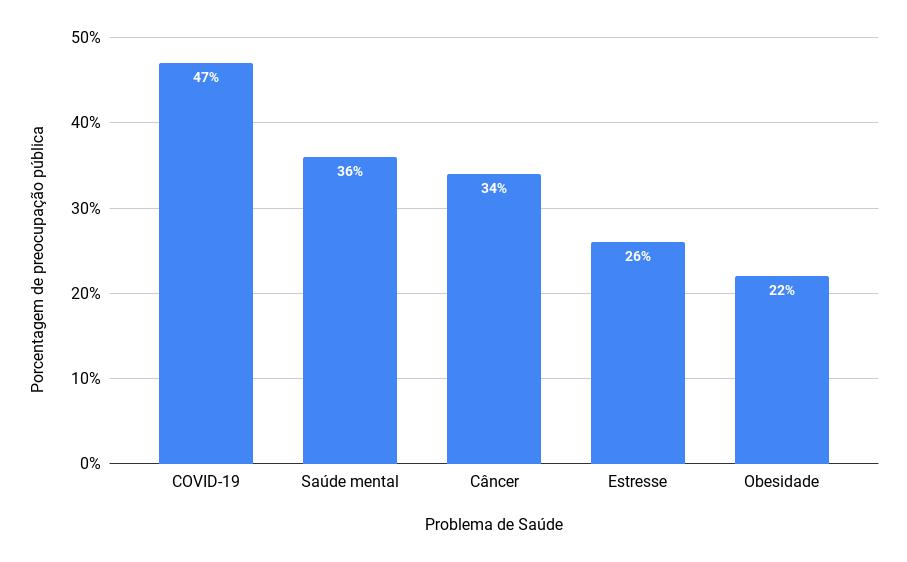
\includegraphics[width=.8\textwidth]{data/figures/interesse-publico.png}
    \fonte{\citeonline{IPSOS2022}}
\end{figure}

Nessa mesma pesquisa constata-se também que dos 34 países incluídos, o Brasil é o sétimo país que mais relata preocupação com saúde mental, onde 49\% dos brasileiros entrevistados a consideram como o problema de saúde mais enfrentado no país atualmente, estando muito acima da média global.

\section{Impactos no mercado de psicologia}
\label{sec:impactoPsicologia}

A pesquisa realizada pela \citeonline{ABP2020}, levou em conta médicos psiquiatras ligados à associação e constatou que cerca de 47\% dos entrevistados relataram aumento em seus atendimentos após o início da pandemia, deste grupo, para cerca de um terço dos entrevistados, os atendimentos cresceram em até 25\%.

Diante da perspectiva de aumento, a pesquisa também citou que cerca de 68\% dos entrevistados receberam pacientes novos, que nunca haviam apresentado sintomas psiquiátricos antes. Além disso, 69\% dos profissionais também relataram que voltaram a atender pacientes que já haviam recebido alta médica e que retornaram ao consultório com reincidência de seus sintomas.

Já para o grupo de profissionais que não perceberam aumento em seus atendimentos, cerca de 45\% dos entrevistados discursaram justamente ao movimento contrário, a de queda em seus atendimentos. Dentre os motivos listados, o de maior destaque está na interrupção do tratamento por parte do paciente, devido às problemáticas de contato da pandemia.

Em outro âmbito, a pesquisa \textit{COVID-19 Practitioner Impact Survey}, realizada pela \citeonline{Association2022}, que levou em consideração profissionais licenciados dos Estados Unidos, relatou que cerca de 38\% dos profissionais constataram estar trabalhando mais em relação ao início da pandemia. Nesse mesmo contexto, cerca de 43\% dos entrevistados relataram estarem atendendo mais pacientes em comparação ao período anterior da pandemia, onde em média, 15.7 pessoas contatam o profissional por mês (excluindo os que já são pacientes).

Por fim, segundo a pesquisa, tamanho crescimento do mercado extrapola-se em outra tendência do mercado, cerca de 4 em cada 10 psicólogos (38\%) relatam manter uma lista de espera com tamanhos variados, onde 58\% são listas de até 9 pessoas e 20\% são listas de 10 até 19 pessoas, conforme expõe a \refImage{listaDeEspera}:

\image
    {Número de pessoas em fila de espera para atendimento psicológico}
    {listaDeEspera}
    {data/figures/lista-de-espera-psicologia.png}
    {width=.9\textwidth}
    {\citeonline{Association2022}}
\section{Tendência de integração tecnológica}
\label{sec:tendenciaDeIntegracaoTecnologica}

De acordo com o resumo científico \textit{Mental Health and COVID-19: Early evidence of the pandemic’s impact} publicado pela \citeonline{OMS2022}, a disrupção causada principalmente pela pandemia SARS-CoV-2 levou a profissionais da área de saúde mental relatarem cortes abruptos por inúmeros motivos em acompanhamentos psicológicos de seus pacientes.

Ainda de acordo com o resumo, para mitigar os danos causados pelos cortes, grande parte dos profissionais da área alegaram que passaram a integrar em seus serviços tecnologias digitais, com consultas, terapias e acompanhamentos pelo telefone ou por meio de plataformas de videoconferência e aplicações \textit{web}.

Essa migração provou-se ser mais flexível e assertiva para grupos específicos de pessoas, em especial pessoas mais novas e/ou financeiramente independentes com seu próprio espaço privado. Além disso, diversas revisões coletadas pelo resumo também relatam avaliações positivas dessa mudança em termos de custo-efetividade, aceitabilidade e conveniência, especialmente para transtornos mentais comuns e para atendimento ambulatorial.
